\documentclass[conference]{IEEEtran}

\usepackage{cite}
\usepackage{amsmath,amssymb}
\usepackage{booktabs}
\usepackage{array}
\usepackage{siunitx}
\usepackage{pgfplots}
\usepackage{url}
\usepackage[hidelinks]{hyperref}

\pgfplotsset{compat=1.18}
\sisetup{round-mode=places,round-precision=3}
\newcolumntype{L}[1]{>{\raggedright\arraybackslash}p{#1}}
\emergencystretch=2em

\begin{document}

\title{When FLOPs Mislead: Benchmarking Neural Network Inference Energy on Apple Silicon}

\author{
\IEEEauthorblockN{Aryan Shah}
\IEEEauthorblockA{Texas Academy of Mathematics and Science\\
University of North Texas\\
Denton, TX, USA\\
aryanshah.2431@gmail.com}
\and
\IEEEauthorblockN{Romir Kadiam}
\IEEEauthorblockA{Texas Academy of Mathematics and Science\\
University of North Texas\\
Denton, TX, USA\\
romirkadiam123@gmail.com}
}

\maketitle

\begin{abstract}
Energy is a deployment constraint for edge-AI systems, but neural-network
efficiency is still often discussed using architecture-level proxies such as
FLOPs, parameter count, and model size. We benchmark five image-classification
architectures on Apple Silicon under CPU-only PyTorch inference and compare
measured per-inference energy, latency, FLOPs, and Energy-Delay Product (EDP).
In the primary five-model mean table, latency almost completely explains
between-model energy variation ($R^2=0.99999$), while FLOPs explains almost
none ($R^2=0.00008$). EfficientNet-B0 consumes $2.65\times$ the energy of
ResNet-18 despite having $4.7\times$ fewer FLOPs. Separate 50-window
\texttt{powermetrics} audits on Apple M1, Apple M4 Pro, and Apple M5 Pro
preserve the qualitative pattern: latency remains strongly predictive of
measured energy ($R^2=0.996$, $0.980$, and $0.975$), while FLOPs remains
uninformative ($R^2=0.001$, $0.001$, and $0.005$). We also
summarize a residualized conditional WGAN-GP used only as supplemental
support for sparse repeated-trial analysis. The results support a practical
benchmarking lesson for embedded and edge inference: direct latency and power
measurement are more informative than FLOP counts alone under a fixed runtime
and input shape.
\end{abstract}

\begin{IEEEkeywords}
edge AI, benchmarking, neural network inference, energy measurement, Apple
Silicon, energy-delay product
\end{IEEEkeywords}

\section{Introduction}

High-performance embedded and edge systems increasingly run neural-network
inference under strict energy and latency budgets. Model selection is often
guided by FLOPs, parameter count, or model size because these quantities are
easy to compute before deployment. They are useful descriptors, but they do
not directly measure wall-clock work, memory traffic, kernel efficiency, or
the behavior of a specific runtime on a specific processor
\cite{horowitz2014,eyeriss2017,hardwareaware2019}.

This paper studies a narrow but practical question: for a fixed Apple Silicon
CPU-only PyTorch runtime, which common architecture proxy best tracks measured
inference energy? The answer in this benchmark is latency, not FLOPs. This is
important for HPEC-style edge deployments because the relevant cost is the
energy actually paid by the hardware under the deployment runtime, not the
nominal arithmetic count of the neural network.

The contributions are:
\begin{itemize}
\item A five-architecture Apple-Silicon inference-energy benchmark comparing
MobileNetV3-Small, MobileNetV2, ResNet-18, Tiny-ViT-5M, and EfficientNet-B0.
\item Direct 50-window \texttt{powermetrics} audits from Apple M1, Apple
M4 Pro, and Apple M5 Pro, with raw logs, per-window inference counts,
confidence intervals, and environment metadata.
\item A compact analysis showing that latency is a much stronger predictor of
energy than FLOPs in the original mean table and in the repeated audits.
\item A scoped synthetic-trial modeling note: residualized conditional GANs
can support exploratory repeated-trial analysis, but they should not replace
independent power measurements.
\end{itemize}

The goal is not to crown one architecture as universally best. The benchmark
is fixed-input and fixed-runtime. It asks what happens when common
architecture families are deployed through the same CPU backend, and whether
the usual complexity proxies preserve the measured energy ordering.

\section{Related Work}

Efficient neural-network design has produced architectures such as MobileNet,
MobileNetV2, MobileNetV3, EfficientNet, SqueezeNet, and ShuffleNet, which
reduce arithmetic through depthwise separable convolutions, inverted
residuals, compound scaling, and channel grouping
\cite{mobilenet2017,mobilenetv22018,mobilenetv32019,efficientnet2019,
squeezenet2016,shufflenet2018}. These designs often improve accuracy/FLOP
tradeoffs, but hardware energy depends on more than FLOPs.

Prior systems work shows that data movement and memory hierarchy behavior can
dominate arithmetic energy \cite{horowitz2014,eyeriss2017}. Hardware-aware
model design similarly emphasizes that latency and hardware utilization can
diverge from FLOP counts \cite{hardwareaware2019,mnasnet2019,fbnet2019}.
Green AI and ML systems benchmarking further motivate reporting measured
deployment costs rather than abstract complexity alone
\cite{greenai2020,strubell2019,patterson2021,mlperf2020}. This paper adds a
small, auditable Apple-Silicon case study centered on per-inference energy.

\section{Methodology}

\subsection{Runtime and Hardware Scope}

All primary results use CPU-only PyTorch inference with batch size 1 and input
shape $1\times3\times224\times224$. CPU-only execution was chosen to isolate a
portable runtime path and avoid Neural Engine or Metal scheduling effects. It
does not claim to be the most energy-efficient Apple Silicon backend.

The repository contains four Apple-Silicon energy sources. The first is the
paper-aligned original five-model mean table, which reports one mean
latency and one mean energy per model from Apple-Silicon CPU inference
measured with \texttt{powermetrics} at 1 Hz. The raw logs for that original
mean table are unavailable, so we do not infer confidence intervals for it.
The other sources are later direct audits: one Apple M1 run, one Apple M4 Pro
run, and one Apple M5 Pro run. Each audit uses 10 20-second windows per
model, 50 windows total, 1 Hz \texttt{powermetrics} sampling, 10 warmup
inferences, and randomized model order.

\begin{table}[t]
\centering
\caption{Direct repeated energy-audit environments.}
\label{tab:env}
\scriptsize
\setlength{\tabcolsep}{2pt}
\begin{tabular}{llll}
\toprule
Audit & Chip/RAM & OS & Python/PyTorch \\
\midrule
M1 & Apple M1 / 8 GB & 26.3 & 3.12.1 / 2.12.0 \\
M4 & M4 Pro / 24 GB & 26.2 & 3.9.6 / 2.8.0 \\
M5 & M5 Pro / 24 GB & 26.4.1 & 3.12.1 / 2.3.1 \\
\bottomrule
\end{tabular}
\end{table}

The original mean table and the direct audits are intentionally kept separate.
The first supports the main comparison used in the earlier manuscript; the
later audits supply raw logs and repeated-window uncertainty for newer local
environments. All three direct audits use one CPU thread, batch size 1,
20-second windows, and the same randomized model order seed. Agreement among
them is therefore treated as robustness of the qualitative pattern rather than
identity of absolute energy values.

\subsection{Metrics}

We report per-inference energy $E$ in joules, latency $L$ in milliseconds,
and average power $P=1000E/L$. Because power is sampled once per second,
energy is interpreted as window-level energy divided by the number of
inferences completed in the window. We also report Energy-Delay Product
(EDP), a standard low-power metric:
\begin{equation}
\mathrm{EDP}=E\cdot L .
\end{equation}
EDP is not accuracy-normalized; it measures energy-latency cost for fixed
input-shape inference.

\subsection{Benchmark Procedure}

The measurement workflow is designed to separate model execution from power-log
parsing. Each model is instantiated once, switched to evaluation mode, and run
with gradients disabled. Warmup inferences are discarded so that module loading
and one-time kernel setup do not dominate short windows. During each measured
window, the script repeatedly executes forward passes until the window expires,
records the number of completed inferences, and then divides the package-energy
estimate for that same window by the inference count. The raw
\texttt{powermetrics} output is retained, so the summary CSV is not the only
source of evidence.

This windowed procedure is deliberately conservative for sub-100 ms inference.
It does not try to attribute a single instantaneous power sample to one forward
pass. Instead, it measures many repeated inferences under a controlled loop and
reports the average energy paid by that loop. This matches the operating mode of
many embedded inference services, where steady-state throughput and energy per
request are more relevant than the energy of a single isolated call.

Table~\ref{tab:checks} lists the main validity checks used when interpreting
the benchmark. These checks are simple, but they make the artifact easier to
audit: the paper distinguishes measured quantities from proxies, reports the
exact hardware and software stack, and avoids using synthetic samples as
physical measurements.

\begin{table}[t]
\centering
\caption{Benchmark validity checks used in the HPEC artifact.}
\label{tab:checks}
\small
\begin{tabular}{L{0.37\linewidth}L{0.53\linewidth}}
\toprule
Risk & Mitigation \\
\midrule
Startup overhead & discard warmup inferences before each measured window \\
Order effects & randomize model order with a recorded seed \\
Power-log ambiguity & retain raw \texttt{powermetrics} logs and window counts \\
Proxy confusion & label latency-only sweep energy as proxy and exclude it from direct-energy claims \\
Synthetic overclaiming & evaluate WGAN-GP separately and treat it as supplemental only \\
\bottomrule
\end{tabular}
\end{table}

\subsection{Supplemental Synthetic Modeling}

The repository includes a conditional WGAN-GP pipeline used to explore
synthetic repeated trials under sparse measurement budgets. An initial
multi-device raw-scale model mode-collapsed. The revised model uses
within-combination residuals: for each device/model combination $c$ and
feature $x$, the training value is
\begin{equation}
\tilde{x}=\mathrm{clip}\left((x-\mu_c)/\sigma_c,-3,3\right).
\end{equation}
Generated residuals are mapped back using the same $\mu_c$ and $\sigma_c$.
This synthetic component is treated as supplemental. It can reproduce grounded
means and rankings, but its spreads are not a substitute for held-out measured
trial-level energy data.

The paper also includes a 17-architecture CPU-only latency sweep. That sweep
has 30 measured latency trials per architecture and exact runtime metadata,
but its energy and EDP columns are constant-power proxies rather than direct
energy measurements. We use it only to contextualize latency behavior across
additional small architectures; all energy claims in this paper come from
the five-model measured energy tables.

\section{Results}

Table~\ref{tab:primary} summarizes the five-model paper-aligned original
mean table.
The key result is that energy follows latency rather than FLOPs. EfficientNet
B0 has only 0.39 GFLOPs, but it has the largest latency and energy. ResNet-18
has 1.82 GFLOPs, yet consumes less than half the energy of EfficientNet-B0 in
this setup.

\begin{table}[t]
\centering
\caption{Paper-aligned original five-model mean table. EDP is
lower-is-better and is computed from measured energy and latency.}
\label{tab:primary}
\small
\begin{tabular}{lrrrr}
\toprule
Model & FLOPs & Lat. & Energy & EDP\\
 & (G) & (ms) & (J) & (J$\cdot$ms)\\
\midrule
MobileNetV3-S & 0.22 & 15.14 & 0.080 & 1.211\\
MobileNetV2 & 0.30 & 20.07 & 0.106 & 2.127\\
ResNet-18 & 1.82 & 20.68 & 0.110 & 2.275\\
Tiny-ViT-5M & 1.30 & 41.33 & 0.219 & 9.051\\
EfficientNet-B0 & 0.39 & 55.08 & 0.292 & 16.083\\
\bottomrule
\end{tabular}
\end{table}

The ordering is monotone in latency and not monotone in FLOPs. MobileNetV3
Small is the lowest-energy model and EfficientNet-B0 is the highest-energy
model. ResNet-18 is the clearest counterexample to a FLOP-based story: it has
the largest FLOP count in the set but remains close to MobileNetV2 in latency
and energy. EfficientNet-B0 has substantially fewer FLOPs than ResNet-18, yet
it takes longer and consumes more energy.

\subsection{Predictor Analysis}

We fit univariate linear models predicting energy from latency, FLOPs, and
parameter count. Table~\ref{tab:predictors} shows that latency explains nearly
all measured energy variation in the five-model mean table, while FLOPs and
parameters do not. Leave-one-out checks preserve the same qualitative result:
latency $R^2$ ranges from 0.99997 to 0.999999, while FLOPs ranges from 0.028
to 0.207.

\begin{table}[t]
\centering
\caption{Univariate predictors of energy in the paper-aligned mean table
($n=5$).}
\label{tab:predictors}
\small
\begin{tabular}{lrr}
\toprule
Predictor & $R^2$ & Pearson $r$\\
\midrule
Latency (ms) & 0.99999 & 0.99999\\
FLOPs (G) & 0.00008 & -0.009\\
Parameters (M) & 0.0547 & 0.234\\
\bottomrule
\end{tabular}
\end{table}

\begin{figure}[t]
\centering
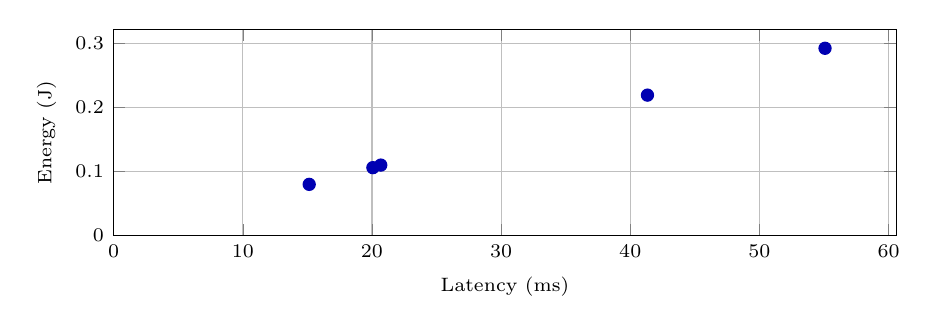
\begin{tikzpicture}
\begin{axis}[
    width=0.95\linewidth,
    height=4.2cm,
    xlabel={Latency (ms)},
    ylabel={Energy (J)},
    xmin=0,
    ymin=0,
    grid=both,
    tick label style={font=\scriptsize},
    label style={font=\scriptsize},
]
\addplot[only marks,mark=*,mark size=2.2pt,color=blue!70!black] coordinates {
    (15.14,0.080)
    (20.07,0.106)
    (20.68,0.110)
    (41.33,0.219)
    (55.08,0.292)
};
\end{axis}
\end{tikzpicture}
\caption{Measured energy versus latency in the five-model mean table.
Latency gives $R^2=0.99999$.}
\label{fig:energy-latency}
\end{figure}

\begin{figure}[t]
\centering
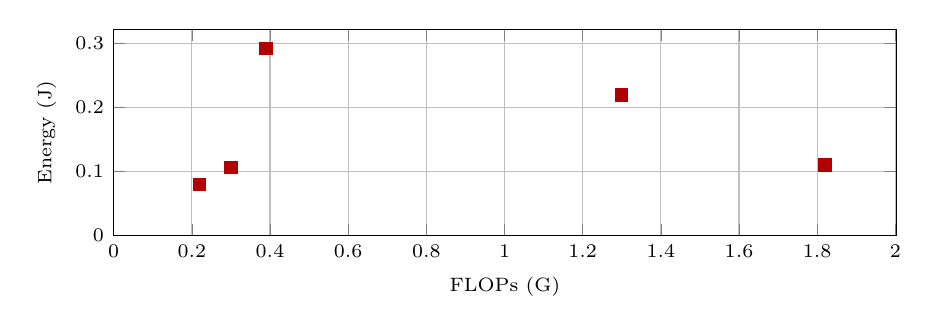
\begin{tikzpicture}
\begin{axis}[
    width=0.95\linewidth,
    height=4.2cm,
    xlabel={FLOPs (G)},
    ylabel={Energy (J)},
    xmin=0,
    ymin=0,
    grid=both,
    tick label style={font=\scriptsize},
    label style={font=\scriptsize},
]
\addplot[only marks,mark=square*,mark size=2.2pt,color=red!70!black] coordinates {
    (0.22,0.080)
    (0.30,0.106)
    (1.82,0.110)
    (1.30,0.219)
    (0.39,0.292)
};
\end{axis}
\end{tikzpicture}
\caption{Measured energy versus FLOPs in the same table. FLOPs gives
$R^2=0.00008$ and ranks some models in the wrong direction.}
\label{fig:energy-flops}
\end{figure}

\subsection{Repeated Energy Audits}

Figure~\ref{fig:audit-energy} reports
separate direct \texttt{powermetrics} audits on
Apple M1, M4 Pro, and M5 Pro systems. Absolute values differ from the original
paper-aligned mean table because the audits were collected later on specific
local environments. They are therefore used as repeatability evidence, not as
retroactive uncertainty estimates for the original table. Still, the same
pattern holds: latency explains most between-model energy variation
($R^2=0.996$ on M1, $0.980$ on M4 Pro, and $0.975$ on M5 Pro), while FLOPs
remains weak ($R^2=0.001$, $0.001$, and $0.005$).
\begin{figure*}[t]
\centering
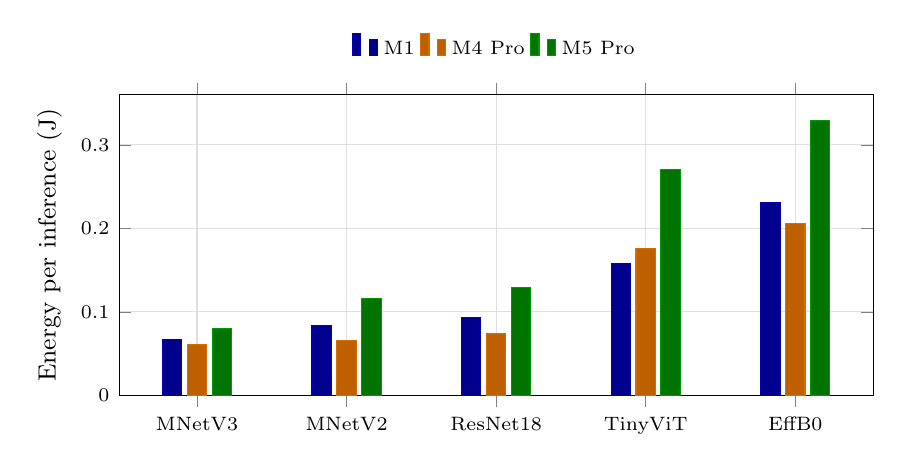
\begin{tikzpicture}
\begin{axis}[
    width=0.92\textwidth,
    height=5.4cm,
    ybar,
    bar width=7pt,
    ymin=0,
    ymax=0.36,
    ylabel={Energy per inference (J)},
    symbolic x coords={MNetV3,MNetV2,ResNet18,TinyViT,EffB0},
    xtick=data,
    enlarge x limits=0.13,
    grid=both,
    major grid style={draw=gray!25},
    tick label style={font=\scriptsize},
    label style={font=\small},
    legend style={
        at={(0.5,1.08)},
        anchor=south,
        legend columns=3,
        draw=none,
        font=\scriptsize
    },
]
\addplot+[fill=blue!55!black,draw=blue!70!black] coordinates {
    (MNetV3,0.067) (MNetV2,0.084) (ResNet18,0.093)
    (TinyViT,0.158) (EffB0,0.231)
};
\addplot+[fill=orange!75!black,draw=orange!85!black] coordinates {
    (MNetV3,0.061) (MNetV2,0.066) (ResNet18,0.074)
    (TinyViT,0.176) (EffB0,0.206)
};
\addplot+[fill=green!45!black,draw=green!60!black] coordinates {
    (MNetV3,0.080) (MNetV2,0.116) (ResNet18,0.129)
    (TinyViT,0.270) (EffB0,0.329)
};
\legend{M1,M4 Pro,M5 Pro}
\end{axis}
\end{tikzpicture}
\caption{Mean per-inference energy across the three 50-window
\texttt{powermetrics} audits. The plotted values come directly from the
summary CSVs; the repository retains the corresponding confidence intervals,
latencies, power estimates, per-window trials, and raw logs.}
\label{fig:audit-energy}
\end{figure*}

The repeated audits expose measurement variability that the original mean
table cannot provide. The M1 audit is slower but lower-power than the newer
Pro-chip audits, so its energy is competitive on several models despite higher
latency. The M5 Pro audit has higher measured average power than the M4 Pro
audit under this CPU-only PyTorch configuration, so its per-inference energies
are often higher even when latency is similar. This should not be read as a
universal hardware-efficiency ordering: the machines also differ in run
timing, OS version, Python version, and PyTorch version. What is stable across
the audits is the architecture ranking:
MobileNetV3-Small, MobileNetV2, and ResNet-18 form a low-energy group, while
Tiny-ViT-5M and EfficientNet-B0 are higher-energy under this CPU runtime.

\subsection{Expanded Latency Sweep}

The 17-architecture latency sweep broadens the performance context without
making new direct energy claims. Table~\ref{tab:latency-sweep} spans very
small MLPs, patch mixers, plain CNNs, depthwise CNNs, grouped convolutions,
residual CNNs, attention-gated CNNs, and ConvNeXt-like blocks. The sweep shows
that latency can vary by orders of magnitude even when FLOPs are small, which
is consistent with the direct-energy finding that runtime behavior matters.

\begin{table*}[t]
\centering
\caption{Full 17-architecture direct latency sweep. Energy values in
that sweep are excluded here because they are constant-power proxies, not
direct \texttt{powermetrics} measurements.}
\label{tab:latency-sweep}
\scriptsize
\begin{tabular}{llrrrrr}
\toprule
Architecture & Family & Params & FLOPs & Lat. & P95 Lat. & CV\\
 & & (M) & (G) & (ms) & (ms) & \\
\midrule
Global avg. MLP tiny & MLP & 0.065 & 0.0001 & 0.026 & 0.026 & 0.013\\
Patch mixer small & Mixer & 0.224 & 0.0419 & 0.465 & 0.528 & 0.071\\
Patch mixer medium & Mixer & 0.435 & 0.1013 & 0.792 & 0.866 & 0.056\\
CNN tiny 2conv & Plain CNN & 0.038 & 0.0398 & 0.793 & 0.836 & 0.029\\
CNN small 4conv & Plain CNN & 0.112 & 0.1699 & 1.306 & 1.375 & 0.032\\
Depthwise small & Depthwise CNN & 0.053 & 0.0233 & 1.446 & 1.508 & 0.027\\
Grouped conv CNN & Grouped CNN & 0.154 & 0.1713 & 1.924 & 2.137 & 0.064\\
Depthwise medium & Depthwise CNN & 0.112 & 0.0501 & 1.998 & 2.111 & 0.051\\
Attention gate CNN & Attention CNN & 0.179 & 0.5260 & 2.373 & 2.428 & 0.014\\
CNN medium 6conv & Plain CNN & 0.482 & 0.7463 & 2.416 & 2.497 & 0.020\\
Squeeze-expand CNN & Squeeze CNN & 0.173 & 0.5967 & 3.114 & 3.219 & 0.016\\
Residual CNN small & Residual CNN & 0.177 & 1.0623 & 3.331 & 3.484 & 0.038\\
Inverted residual small & Inverted residual & 0.080 & 0.2792 & 3.366 & 3.463 & 0.019\\
Bottleneck residual & Bottleneck CNN & 0.227 & 0.7244 & 3.480 & 3.639 & 0.026\\
Inverted residual wide & Inverted residual & 0.167 & 0.8118 & 6.739 & 6.858 & 0.014\\
Residual CNN medium & Residual CNN & 0.514 & 3.4142 & 6.848 & 8.531 & 0.173\\
ConvNeXt micro & ConvNeXt-like & 0.240 & 0.4482 & 7.554 & 7.793 & 0.022\\
\bottomrule
\end{tabular}
\end{table*}

This sweep is useful for systems interpretation. For example, the depthwise
small model has fewer FLOPs than a tiny two-convolution CNN but higher latency,
which is consistent with lower arithmetic intensity and less efficient CPU
kernels. Patch-mixer models are also fast at low arithmetic counts, while the
ConvNeXt-like micro model is slower than several architectures with larger
FLOP counts. The result is not direct energy evidence, but it helps explain why
FLOPs alone should not be used to infer energy on this platform.

\subsection{Synthetic Model Fidelity}

The residualized WGAN-GP is evaluated only as a supplemental modeling tool.
Table~\ref{tab:gan} summarizes the paper-aligned synthetic fidelity against
the grounded Apple-only distribution. Energy and latency pass Kolmogorov--
Smirnov checks at $p>0.05$, and the synthetic means preserve the measured
energy ranking. The strongest claim is therefore limited: the synthetic model
can reproduce the grounded distribution used to train it. It does not prove
physical variance without independent repeated measurements.

\begin{table}[t]
\centering
\caption{Supplemental GAN fidelity against grounded Apple-only data.}
\label{tab:gan}
\small
\begin{tabular}{lrrr}
\toprule
Feature & Wasserstein & KS & $p$\\
\midrule
Energy & 0.0039 & 0.064 & 0.156\\
Latency & 0.6934 & 0.067 & 0.120\\
Derived power & 0.0457 & 0.047 & 0.498\\
\bottomrule
\end{tabular}
\end{table}

\section{Discussion}

The main practical conclusion is not that FLOPs are useless. FLOPs still
describe arithmetic scale, and they are often useful for first-pass model
screening. The conclusion is that FLOPs are insufficient as an energy proxy
for a specific deployment stack. On Apple Silicon CPU-only PyTorch inference,
latency captures backend effects that FLOPs miss: memory traffic, kernel
selection, vectorization, depthwise-convolution efficiency, attention
implementation, and cache behavior.

The architecture comparisons illustrate this. MobileNet-style depthwise
convolutions reduce arithmetic, but on a general-purpose CPU they can become
memory-bound. EfficientNet-B0 has fewer FLOPs than ResNet-18, but its compound
scaling and operator mix produce longer latency. Tiny-ViT-5M has fewer FLOPs
than ResNet-18 but pays for attention and projection operations that are less
friendly to this CPU runtime. These effects are familiar in hardware-aware
model design, but this benchmark shows their impact on measured energy in a
small Apple-Silicon edge-inference case study.

The synthetic GAN results should be interpreted cautiously. The residualized
GAN reproduced measured means within a few percent in the repository workflow,
but it was trained against grounded samples derived from measured means. This
supports sensitivity analysis and artifact generation, not independent
physical validation. HPEC-style benchmarking should prioritize direct power
logs and only use synthetic trials as clearly labeled supplemental data.

The results suggest three practical rules for edge-inference benchmarking.
First, report latency next to energy even when energy is the headline metric,
because latency captures much of the backend behavior that FLOPs hide. Second,
do not compare architectures using FLOPs alone when the operator mix changes:
depthwise convolutions, attention blocks, and compound-scaled CNNs can have
very different CPU efficiency at similar arithmetic counts. Third, preserve
enough raw measurement state for others to audit the result. A single summary
table is hard to diagnose; raw power logs, window durations, inference counts,
thread settings, and hardware metadata make the benchmark substantially more
useful.

For HPEC, the strongest aspect of the work is the benchmark artifact rather
than the GAN. The raw audit logs, randomized model order, window counts, and
environment JSON make the repeated energy audit inspectable. The GAN is still
useful because it documents a failure mode: raw-scale multi-device training
collapsed toward averages, while combo-normalized residual training preserved
within-combination structure. That lesson is relevant for hardware-behavior
modeling, where between-device variation can swamp the effect being studied.
However, any deployment recommendation should be grounded in direct
measurements.

\section{Deployment Implications}

For an embedded developer choosing between candidate networks, the benchmark
supports a measurement-first workflow. FLOPs can narrow the design space, but a
small deployment harness should then measure latency and power under the exact
runtime that will ship. This is especially important when candidates use
different operator families. A dense residual CNN, a depthwise CNN, and a
Transformer-like vision model can present similar arithmetic budgets to a
spreadsheet while exercising the CPU backend very differently.

The result also affects how model-compression work should be reported. A
compressed architecture with fewer FLOPs is not automatically a lower-energy
architecture on a general-purpose CPU. If compression changes the operator mix
toward kernels with poor vectorization or poor cache reuse, wall-clock time can
increase enough to erase the arithmetic gain. Conversely, a model with more
nominal arithmetic can be competitive if the runtime executes its kernels
efficiently. This helps explain why ResNet-18 is not the highest-energy model
in our five-model set despite having the most FLOPs.

For HPEC-style systems papers, this suggests that benchmark artifacts should
include the runtime controls that determine whether results are comparable:
thread count, batch size, input shape, warmup policy, sampling interval,
hardware identifier, software versions, and whether accelerators were enabled.
Without those controls, energy comparisons can become statements about hidden
runtime choices rather than about the architecture being evaluated.

\subsection{External Embedded Reference Points}

Table~\ref{tab:external} gives non-Apple reference points from public embedded
benchmarks: Coral Edge TPU \cite{coralbench,coralfaq}, PyTorch Raspberry Pi
\cite{pytorchrpi}, and STM32 AI Model Zoo \cite{stm32zoo}. These rows are not
used in the Apple-Silicon regression and should not be read as direct
measurements from our artifact.

\begin{table}[t]
\centering
\caption{External embedded reference points. Energy is included only when it
can be inferred from a reported latency and an explicit published power figure.}
\label{tab:external}
\scriptsize
\setlength{\tabcolsep}{2pt}
\begin{tabular}{L{0.20\linewidth}L{0.20\linewidth}rrL{0.13\linewidth}}
\toprule
Device & Model & Lat. & Energy & Evidence \\
 & & (ms) & (J) & \\
\midrule
Coral TPU & MNetV2 & 2.6 & 0.0052 & inferred\\
R-Pi 4 & MNetV2 & 26.4 & -- & latency\\
R-Pi 4 & RN-18 & 100.3 & -- & latency\\
STM32H747I & MNetV2 & 1118.27 & -- & latency\\
\bottomrule
\end{tabular}
\end{table}

The contrast is useful but limited. Coral's inferred energy uses a published
2 W Edge TPU figure and benchmark latency, while the Raspberry Pi and STM32
rows are latency-only. They therefore strengthen the motivation for
hardware-specific measurement but do not replace our direct Apple-Silicon
power logs.

\section{Difference From FTC Version}

A shorter FTC version of this work focused on the initial Apple-Silicon
five-model comparison and the broad warning that FLOPs can mislead as an
energy proxy. This HPEC version adds a systems-oriented artifact contribution:
three direct 50-window \texttt{powermetrics} audits on Apple M1, M4 Pro, and
M5 Pro; raw power logs and per-window inference counts; explicit environment
metadata; consistency checks tying the manuscript to repository CSVs; and a
cleaner cross-chip comparison figure. The HPEC submission therefore emphasizes
reproducible measurement methodology and hardware-dependent benchmarking
rather than only the original model-ranking observation.

\section{Limitations}

The study is intentionally narrow. It covers five architectures, one input
shape, batch size 1, and CPU-only PyTorch inference. It does not evaluate
Apple Neural Engine, Metal Performance Shaders, GPUs, quantization, or
accuracy-normalized energy. The original five-model mean table lacks raw
power logs; the repository adds later direct audits with raw logs, but those
audits are not the original source run. Finally, 1 Hz power sampling is coarse
relative to per-inference latency, so energy is attributed over windows rather
than instantaneous inference events.

There are also statistical limits. The main predictor analysis has only five
architectures, so exact $R^2$ values should be read as descriptive statistics
for this benchmark rather than universal constants. We include leave-one-out
checks, rank checks, and separate audits, but a stronger HPEC version would
add more direct-energy architectures, hardware backends, and batch sizes. The
current result is best viewed as a reproducible case study showing why FLOP
counts can mislead under one realistic edge-inference stack.

\section{Artifact Availability}

\begin{sloppypar}
The repository includes source code, tables, scripts, raw audit logs, and
metadata at
\url{https://github.com/jubs-2431/which-neural-networks-waste-the-most-energy}.
Key artifacts are the Apple benchmark CSV, the M1, M4 Pro, and M5 Pro
energy-summary CSVs, raw
\texttt{powermetrics} logs, the measurement script, and the measurement
protocol.
\end{sloppypar}

The intended reproduction path is lightweight. The existing CSV artifacts can
be inspected without rerunning privileged power measurement. Repeating the
direct energy audit on macOS requires \texttt{powermetrics}, which asks for
administrator privileges, and writes a new set of window-level logs. The
expanded latency sweep can be rerun without privileged access and provides a
sanity check that the CPU-only runtime and thread settings are configured as
expected. The paper source and compiled HPEC draft are included so that the
tables in this submission can be traced directly back to repository artifacts.

\section{Conclusion}

In this Apple-Silicon CPU-only inference benchmark, measured energy tracks
latency far more closely than FLOPs. The result is visible in the
paper-aligned five-model mean table and in later 50-window direct energy
audits from one Apple M1 run, one Apple M4 Pro run, and one Apple M5 Pro run.
For edge-AI and embedded deployments, the engineering lesson is direct:
benchmark the deployed runtime with auditable power traces, and treat FLOPs as
an incomplete proxy rather than an energy measurement.

\begin{thebibliography}{16}

\bibitem{horowitz2014}
M.~Horowitz, ``Computing's energy problem (and what we can do about it),''
\emph{IEEE Micro}, vol.~34, no.~5, pp.~10--14, 2014.

\bibitem{eyeriss2017}
Y.-H. Chen et al., ``Eyeriss: An energy-efficient reconfigurable accelerator
for deep convolutional neural networks,'' \emph{IEEE J. Solid-State Circuits},
2017.

\bibitem{hardwareaware2019}
Y.~He et al., ``Understanding FLOPs is not enough: A study of hardware-aware
neural networks,'' \emph{arXiv preprint arXiv:1912.01090}, 2019.

\bibitem{mobilenet2017}
A.~G. Howard et al., ``MobileNets: Efficient convolutional neural networks for
mobile vision applications,'' \emph{arXiv preprint arXiv:1704.04861}, 2017.

\bibitem{mobilenetv22018}
M.~Sandler, A.~Howard, M.~Zhu, A.~Zhmoginov, and L.-C. Chen,
``MobileNetV2: Inverted residuals and linear bottlenecks,'' in
\emph{Proc. IEEE Conf. Computer Vision and Pattern Recognition}, 2018.

\bibitem{mobilenetv32019}
A.~Howard et al., ``Searching for MobileNetV3,'' in
\emph{Proc. IEEE Int. Conf. Computer Vision}, 2019.

\bibitem{efficientnet2019}
M.~Tan and Q.~Le, ``EfficientNet: Rethinking model scaling for convolutional
neural networks,'' in \emph{Proc. Int. Conf. Machine Learning}, 2019.

\bibitem{squeezenet2016}
F.~N. Iandola et al., ``SqueezeNet: AlexNet-level accuracy with 50x fewer
parameters and $<$0.5MB model size,'' \emph{arXiv:1602.07360}, 2016.

\bibitem{shufflenet2018}
X.~Zhang et al., ``ShuffleNet: An extremely efficient convolutional neural
network for mobile devices,'' in \emph{Proc. IEEE CVPR}, 2018.

\bibitem{mnasnet2019}
M.~Tan et al., ``MnasNet: Platform-aware neural architecture search for
mobile,'' in \emph{Proc. IEEE CVPR}, 2019.

\bibitem{fbnet2019}
B.~Wu et al., ``FBNet: Hardware-aware efficient ConvNet design via
differentiable neural architecture search,'' in \emph{Proc. IEEE CVPR}, 2019.

\bibitem{greenai2020}
R.~Schwartz et al., ``Green AI,'' \emph{Communications of the ACM}, vol.~63,
no.~12, pp.~54--63, 2020.

\bibitem{strubell2019}
E.~Strubell, A.~Ganesh, and A.~McCallum, ``Energy and policy considerations
for deep learning in NLP,'' in \emph{Proc. ACL}, 2019.

\bibitem{patterson2021}
D.~Patterson et al., ``Carbon emissions and large neural network training,''
\emph{arXiv:2104.10350}, 2021.

\bibitem{mlperf2020}
V.~J. Reddi et al., ``MLPerf inference benchmark,'' in \emph{Proc. ACM/IEEE
ISCA}, 2020.

\bibitem{coralbench}
Google Coral, ``Edge TPU performance benchmarks,'' accessed May 2026.

\bibitem{coralfaq}
Google Coral, ``Frequently asked questions,'' accessed May 2026.

\bibitem{pytorchrpi}
PyTorch, ``Real time inference on Raspberry Pi,'' accessed May 2026.

\bibitem{stm32zoo}
STMicroelectronics, ``STM32 AI model zoo: MobileNetV2,'' accessed May 2026.

\bibitem{wgangp2017}
I.~Gulrajani et al., ``Improved training of Wasserstein GANs,'' in
\emph{Advances in Neural Information Processing Systems}, 2017.

\end{thebibliography}

\end{document}
